\section{Educational Theories}

There are many theories of how people learn, how to teach, and how to engage with students. 
In this section of the proposal, we review dominant theories that guide the research.
First, we will discuss how people learn, and the dominant theories that guide researchers.
Then, we will discuss Instructional Design, which is concerned with how to support the learning process.
Finally, we will look at motivation and engagement, the reason people choose to direct their energy towards goals.

\subsection{Theories of Learning}


There are many, many theories of learning, far more than can be accurately captured here.
However, there are a few major paradigms worth discussing briefly: Cognitivism, Constructivisim, and Behavioralism.
Cognitivism emerged as a response to classical theories on Behaviorist learning -- the latter posits learning as a ``black box'' process, and the former encourages researchers to ``pry open the box'' \cite{learningtheories}.
This in turn led to the development of Constructivism, which describes learning as an active process of linking knowledge based on prior, subjective experiences.
These theories are not replacements for each, but lenses for analyzing different learning experiences. Cognitivism and Constructivism in particular are usually more useful for studying higher learning.

\subsubsection{Situated Learning Theory}

Situated Learning Theory, originally proposed by Lave and Wenger, argues that learning normally occurs as a function of the activity, context, and culture in which it is situated\cite{lave-situated}.
Therefore, tasks in the learning environment should parallel real-world tasks, in order to maximize the \textit{authenticity}.
Contextualization is key in these settings, as opposed to decontextualized (or ``inert'') settings.
The key difference is that learning is driven by the problem being solved, rather than the tools available – therefore, the problem being solved should lead directly to the tool being taught.

A critical element of these situated environments is the need for social interaction and collaboration, as learners become involved in and acculturated by ``Communities of Practice'' \cite{brown1989situated}.
Members of a CoP share purposes, tools, processes, and a general direction -- they should have a commonly recognized domain. 
This interaction occurs not only between individuals and the experts of the community (commonly represented by teachers) in an apprenticeship model, but also occurs between different learners as they adapt at uneven paces.
This communication between peers leads to growth among both individuals, especially when access to authentic experts is limited.
As the learner develops into an expert, they shift from the outside of the community's circle to the center, becoming more and more engaged -- this is the process of ``Legitimate Peripheral Participation''.

Authenticity is another crucial, recurring theme within Situated Learning Theory.
All instruction and assessment must be aligned with reality such that success in the former leads to success in the latter.
However, there is a subtle nuance here -- authenticity is a perceived trait, not an objective one.
Students derive value from their learning only if they \textit{perceive} authenticity, regardless of whether the instructor has successfully authenticated the experience.

Situated Learning Theory has been applied to the domain of Computer Science before, with mixed results. A seminal paper by Ben-Ari \cite{ben2004situated} explores its application and limitations.
This paper is somewhat hasty in its application of SL Theory by taking a macro-level view -- they narrowly look to Open-Source and Industry Software Development communities as the only potential CoPs and interpret SL Theory as strictly requiring constant legitimacy, largely ignoring the possibility for gradual development of authenticity within individual courses and modules throughout a curriculum:

\begin{quote}
What I am claiming is that situated learning as presented in their work cannot be accepted at face value, because it simply ignores the enormous gap between the world of education and the world of high-tech CoPs, which demand extensive knowledge of both CS subjects and applications areas.
This gap can only be bridged by classical decontextualized teaching in high schools, colleges and universities.
\end{quote}

However, other researchers have found it a useful lens for analyzing curricula.
For instance, Guzdial and Tew \cite{guzdial2006imagineering} used the theory to innovatively explore and deal with the problem of inauthenticity within their Media Computation project.
SL Theory clearly has value, but only as a function of the way that it is applied.
In this preliminary proposal, I will take advantage of SL Theory as a generalized tool for exploring the topic of authenticity throughout introductory Computer Science.

The original work in Situated Learning Theory was categorically not about pedagogy or instructional design- it described how people learn and the importance of context and collaboration, but it did not recommend a particular style of classroom.

\subsection{Theories of Instructional Design}

Instructional Design is the systematic design of effective Learning Experiences. One of the most influential\cite{anglin1992reference} instructional theories is Gang\'{e}'s Theory of Instruction, a complex Cognitivist model that categorizes different types of learning outcomes (e.g., ``Verbal Information'' such as reciting the definition of a term, ``Attitudinal'' such as choosing to not smoke) and breaks down the process of learning into nine coherent steps. Gang\'{e} stresses that different learning outcomes require very different instructional implementations of the general instructional model. This instructional theory informs the design of complete Instructional Design models such as the Dick and Carey model \cite{carey2001systematic}. Although different ID models suggest different approaches to creating instructional materials, those materials are all typically patterned after Gang\'{e}'s instructional events.

\subsubsection{Gagn\'{e}'s Instructional Events}

\begin{figure}
\begin{description}
	\item[(1) Gain Attention:] Stimulate the learner and motivate them to engage with the material.
	\item[(2) Describe Objectives:] Inform the learner will be able to do because of the instruction.
	\item[(3) Stimulating Recall of Prior Knowledge:] Remind students of their prior knowledge.
	\item[(4) Present the Material:] Using text, graphics, etc., give the instructional materials.
	\item[(5) Provide Guidance:] Give instructions on how to use the instructional materials.
	\item[(6) Elicit Performance:] Have the learners actively apply the new knowledge.
	\item[(7) Provide Feedback:] Show the learner what they did well and poorly on.
	\item[(8) Assess Performance Test:] Evaluate the learner on their performance
	\item[(9) Enhance Retention and Transfer:] Generalize the instruction by showing similar applications.
\end{description}
\caption{Gang\'{e}'s Nine Events of Instruction}
\label{gange-events}
\end{figure}

Gang\'{e}'s nine events are summarized in Figure \ref{gange-events}, taken indirectly from\cite{gagne1985conditions}. This model is described as an ordered, one-way sequence; however, in practice, some steps might be repeated and cycled between. For instance, very negative feedback might prompt the learner to return from step 7 to step 6. Modifications of the model have also been discussed in the literature. For example, to adapt for more Constructivist tastes, one could swap steps 4 and 6, so that students have the opportunity to engage with the materials before receiving instruction.

Instructional Designers often identify three key interactions in a learning experience. In the simplest case, an instructor presents some new material, a learner participates in questions related to it, and the instructor assesses their performance as being excellent. Although it might appear that Gagn\'{e}'s model maps presentation to steps 1--5, participation to step 6, and assesssment to 7--9, this is an over-simplification of a much richer set of interactions. For instance, step 1 (Gain Attention) often involves a dialogue or other participation from the students, and step 7 often requires re-presentation of existing material or presentation of new material. In practice, every learning experience will end up being a unique combination of these interactions.

Instructors and learners are involved in all of these interactions in different capacities and degrees. Presentation is primarily a flow of information from the Instructor to the learner. Participation is primarily an externalization of knowledge by the learner for the Instructor. Assessment is a mediation between the Instructor and the learner to align the externalization.

Instructional Design Models such as Dick \& Carey usually delay the design of instructional materials till the end of the entire process, focusing initially on analysis of the learners, the performance context, the instructional goal, and a host of other critical factors. At that point, a content delivery system is chosen based on its educational affordances and suitability for the learning experience being developed. This delay reflects the typical role of an Instructional Designer as a \textit{consumer} of instructional technology -- they survey the available techniques and technology (e.g., traditional lecture, essay writing, websites), and choose the one that fits their need. In the remainder of this paper, we use instead take the Software Designer role of \textit{producer} of instructional technology in order to analyze some of the decisions that go into the design of these environments, from the retrospective of an Instructional Designer.

\subsubsection{Situated Learning Environment Design}

Situated Learning Theory is a theory of learning, not a theory of instructional design. However, subsequent research by Brown \cite{brown1989situated} and others expanded the theory so that it could be applied to the design of learning experiences. These expansions often naturally dictate the use of active learning techniques, demphasizing the role of lecture in favor of collaborative, problem-based learning activities.

Choi \& Hannafin \cite{situated-cognition} describe a particularly useful, concrete framework for designing situated learning environments and experiences. Because there is no official name given to this framework, as a matter of convenience we will refer to it as the Situated Learning Environment Design Framework (SLED Framework). This framework has four key principles:

\begin{wrapfigure}{R}{0.5\textwidth}
		\begin{center}
				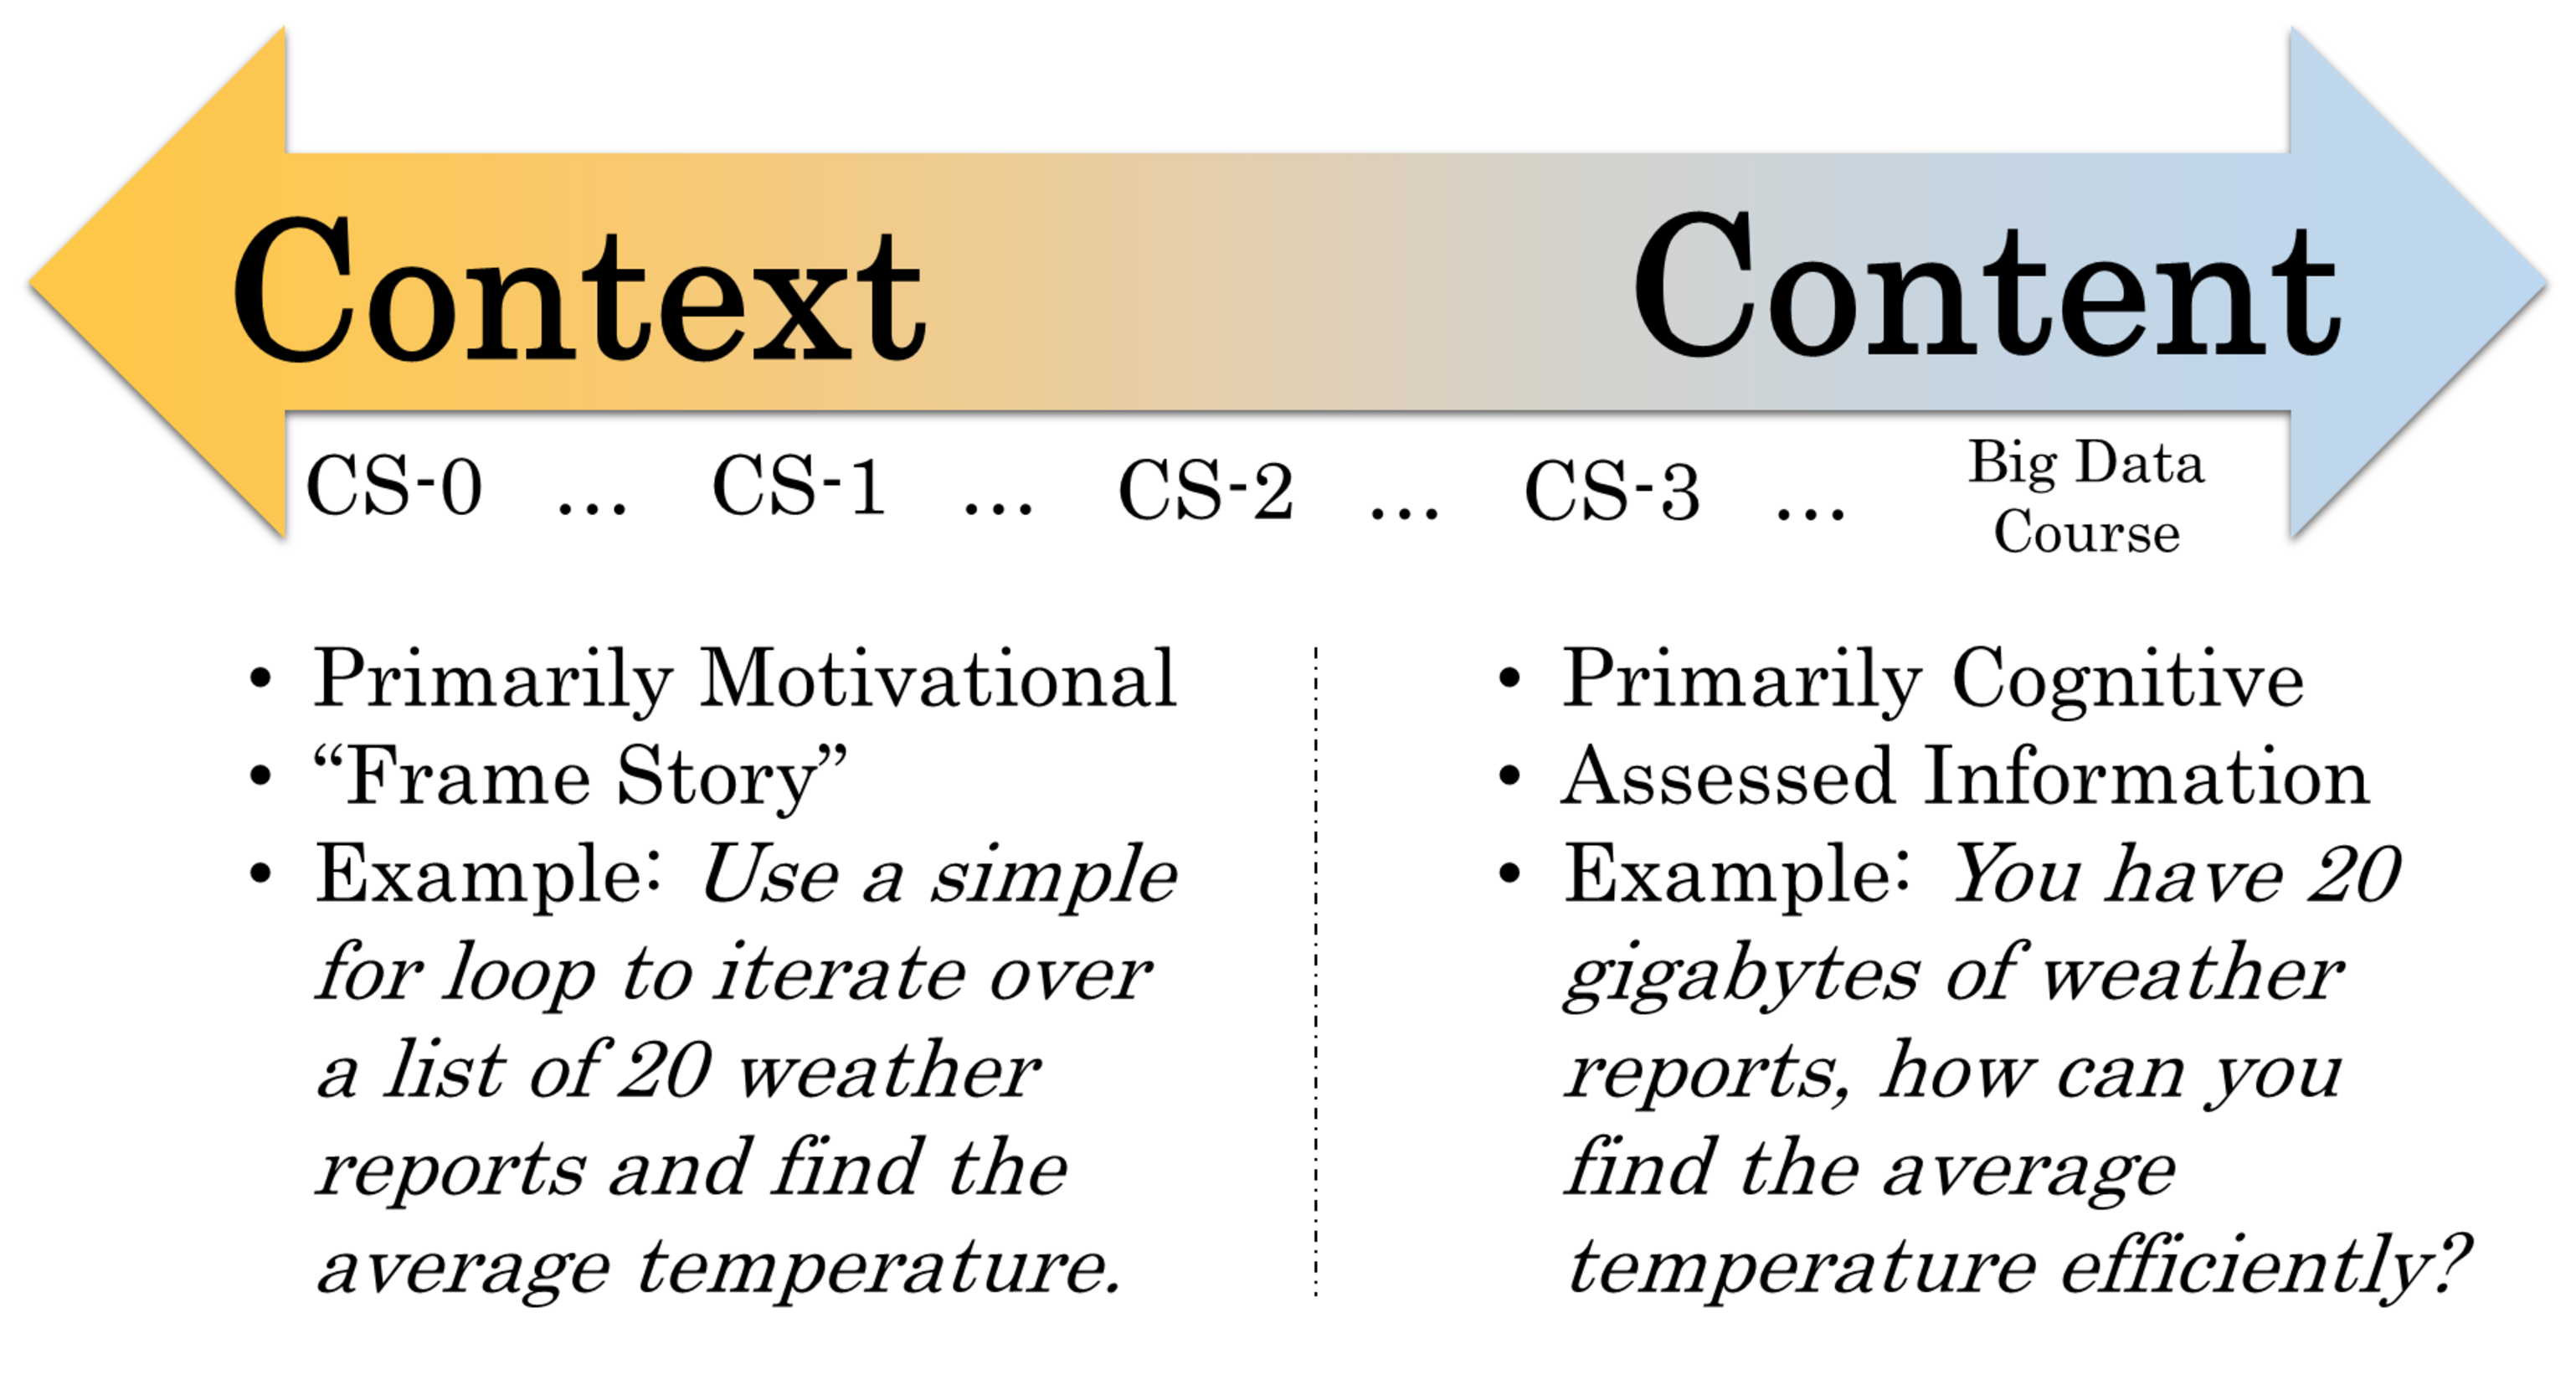
\psfig{file=images/content-context-2.eps, width=\linewidth}
		\end{center}
		\caption{Content vs. Context}
		\label{fig-content-context}
\end{wrapfigure}

\begin{description}
	\item[Context] ``... The problem's physical and conceptual structure as well as the purpose of activity and the social milieu in which it is embedded''\cite{rogoff1984everyday}, context is driven not just by the atmosphere of the problem at hand, but also by the background and culture surrounding the problem.
	A good context enables a student to find recognizable elements and build on prior understanding, eventually being able to freely transfer their learning to new contexts.
	\item[Content] The information intending to be conveyed to the students.
	If context is the backdrop to the learning, then content might be seen as the plot.
	Naturally, context and content are deeply intertwined with each other, and its difficult to talk about one without referencing the other; in fact, content is an abstract entity that needs to be made concrete through contextualization when it is delivered to the learner.
	If the information is too abstract, than it will never connect with the learner and will not be transferable to new domain.
	However, if it is too grounded in a domain, then it will not be clear how it can be re-applied elsewhere. 
	Ultimately, content must be given in a variety of forms to maximize transfer.
	Two useful methods for building content are anchored instruction (exploring scenarios, or anchors, in the context based on the content) and cognitive apprenticeship (mediating knowledge from an expert to the novice learner in a mentoring relationship).
	\item[Facilitations] The modifications to the learning experience that support and accelerate learning.
	Facilitations provide opportunities for students to internalize what they are learning by lowering the barriers that can surround situated experiences, possibly at the cost of some amount of authenticity. 
	These modifications might be technological in nature, but they can also be pedagogical.
	Although there are many different forms that Facilitations can take, Scaffolding is one of the most common.
	Scaffolding is a form of support that is intended to extend what a learner can accomplish on their own.
	This support is required at the onset of the learning process, but is unnecessary once a sufficient threshold has been passed; during this transition, the amount of scaffolding can be tuned to the learners understanding.
	In Computer Science, for instance, students often take advantage of software libraries and frameworks to create sophisticated graphical programs that would be beyond daunting if implemented from scratch.
	\item[Assessment] The methods used to assess the learning experience and the progress of the student.
	Choi \& Hannafin gives special attention to the “teach to the test” problem, and how assessment needs to change to measure students ability to solve authentic problem (as opposed to their ability to solve the test’s specific problem), and to be able to transfer their understanding when solving different but related problems.
	It is important that assessment is measured against the individualized goals and progress of a learner, requiring that any standards used be fluid and adaptable to different learners personal situations.
	Of course, assessment should be an on-going part of the learning process, providing feedback and diagnostics.
	Ultimately, the learner should join in the process of assessment as they transition to an expert – being able to meta-cognitively self-evaluate the effectiveness of ones methods and communicate results to others are key abilities of experts. 
\end{description}

There is a reciprocal relationship between contexts and content.
Figure \ref{fig-content-context} demonstrates an example of this relationship for the expected emphasis on big data as context vs. content throughout an undergraduate curriculum, from a CS-0 (non-majors) course all the way to an upper-level course specifically on big data.
Just as the upper-level course would naturally use big data as its context and content, a CS-0 course could still have content related to big data.
However, the majority of the use of big data would be as the framing story for assignments, especially in earlier parts of the course.
When students learn programming in the context of, say, game development, they are almost necessarily learning content related to game development that may not be universal to computer science -- e.g., how graphical resources are organized and accessed within the game engine.
This content may be seen as a distraction by the instructor, or as useful side knowledge - for example, if a student had to learn how to use a command line in order to compile their game, they would be learning an authentic skill that might not be considered part of the core content, but is nonetheless generally useful.
When evaluating a context, it is useful to consider what content it represents, and how authentic and useful it is.
The authenticity of content that is attached to a context affects the authenticity of the learning environment as a whole.

Fascinatingly, the need for a strong context diminishes as learners mature and become domain-identified -- the content itself becomes the context.
Learners start to see other contexts as nothing more than distractions and unnecessary fluff.
This makes sense -- you would hope that Computer Science majors in their third semester would be naturally interested in the material, and this is borne out in experimental data.
For instance, Yarosh \& Guzdial attempted to integrate Media Computation in a CS-2 (Data Structures) course, and found that the learners had ``outgrown the desire for a context''~\cite{yarosh2008narrating}. 
These results are similar to results we found in our interventions with a CS-3 (Data Structures and Algorithms), where students seemed more irked by the surrounding context than intrigued.

\begin{figure}[!ht]
	\begin{center}
		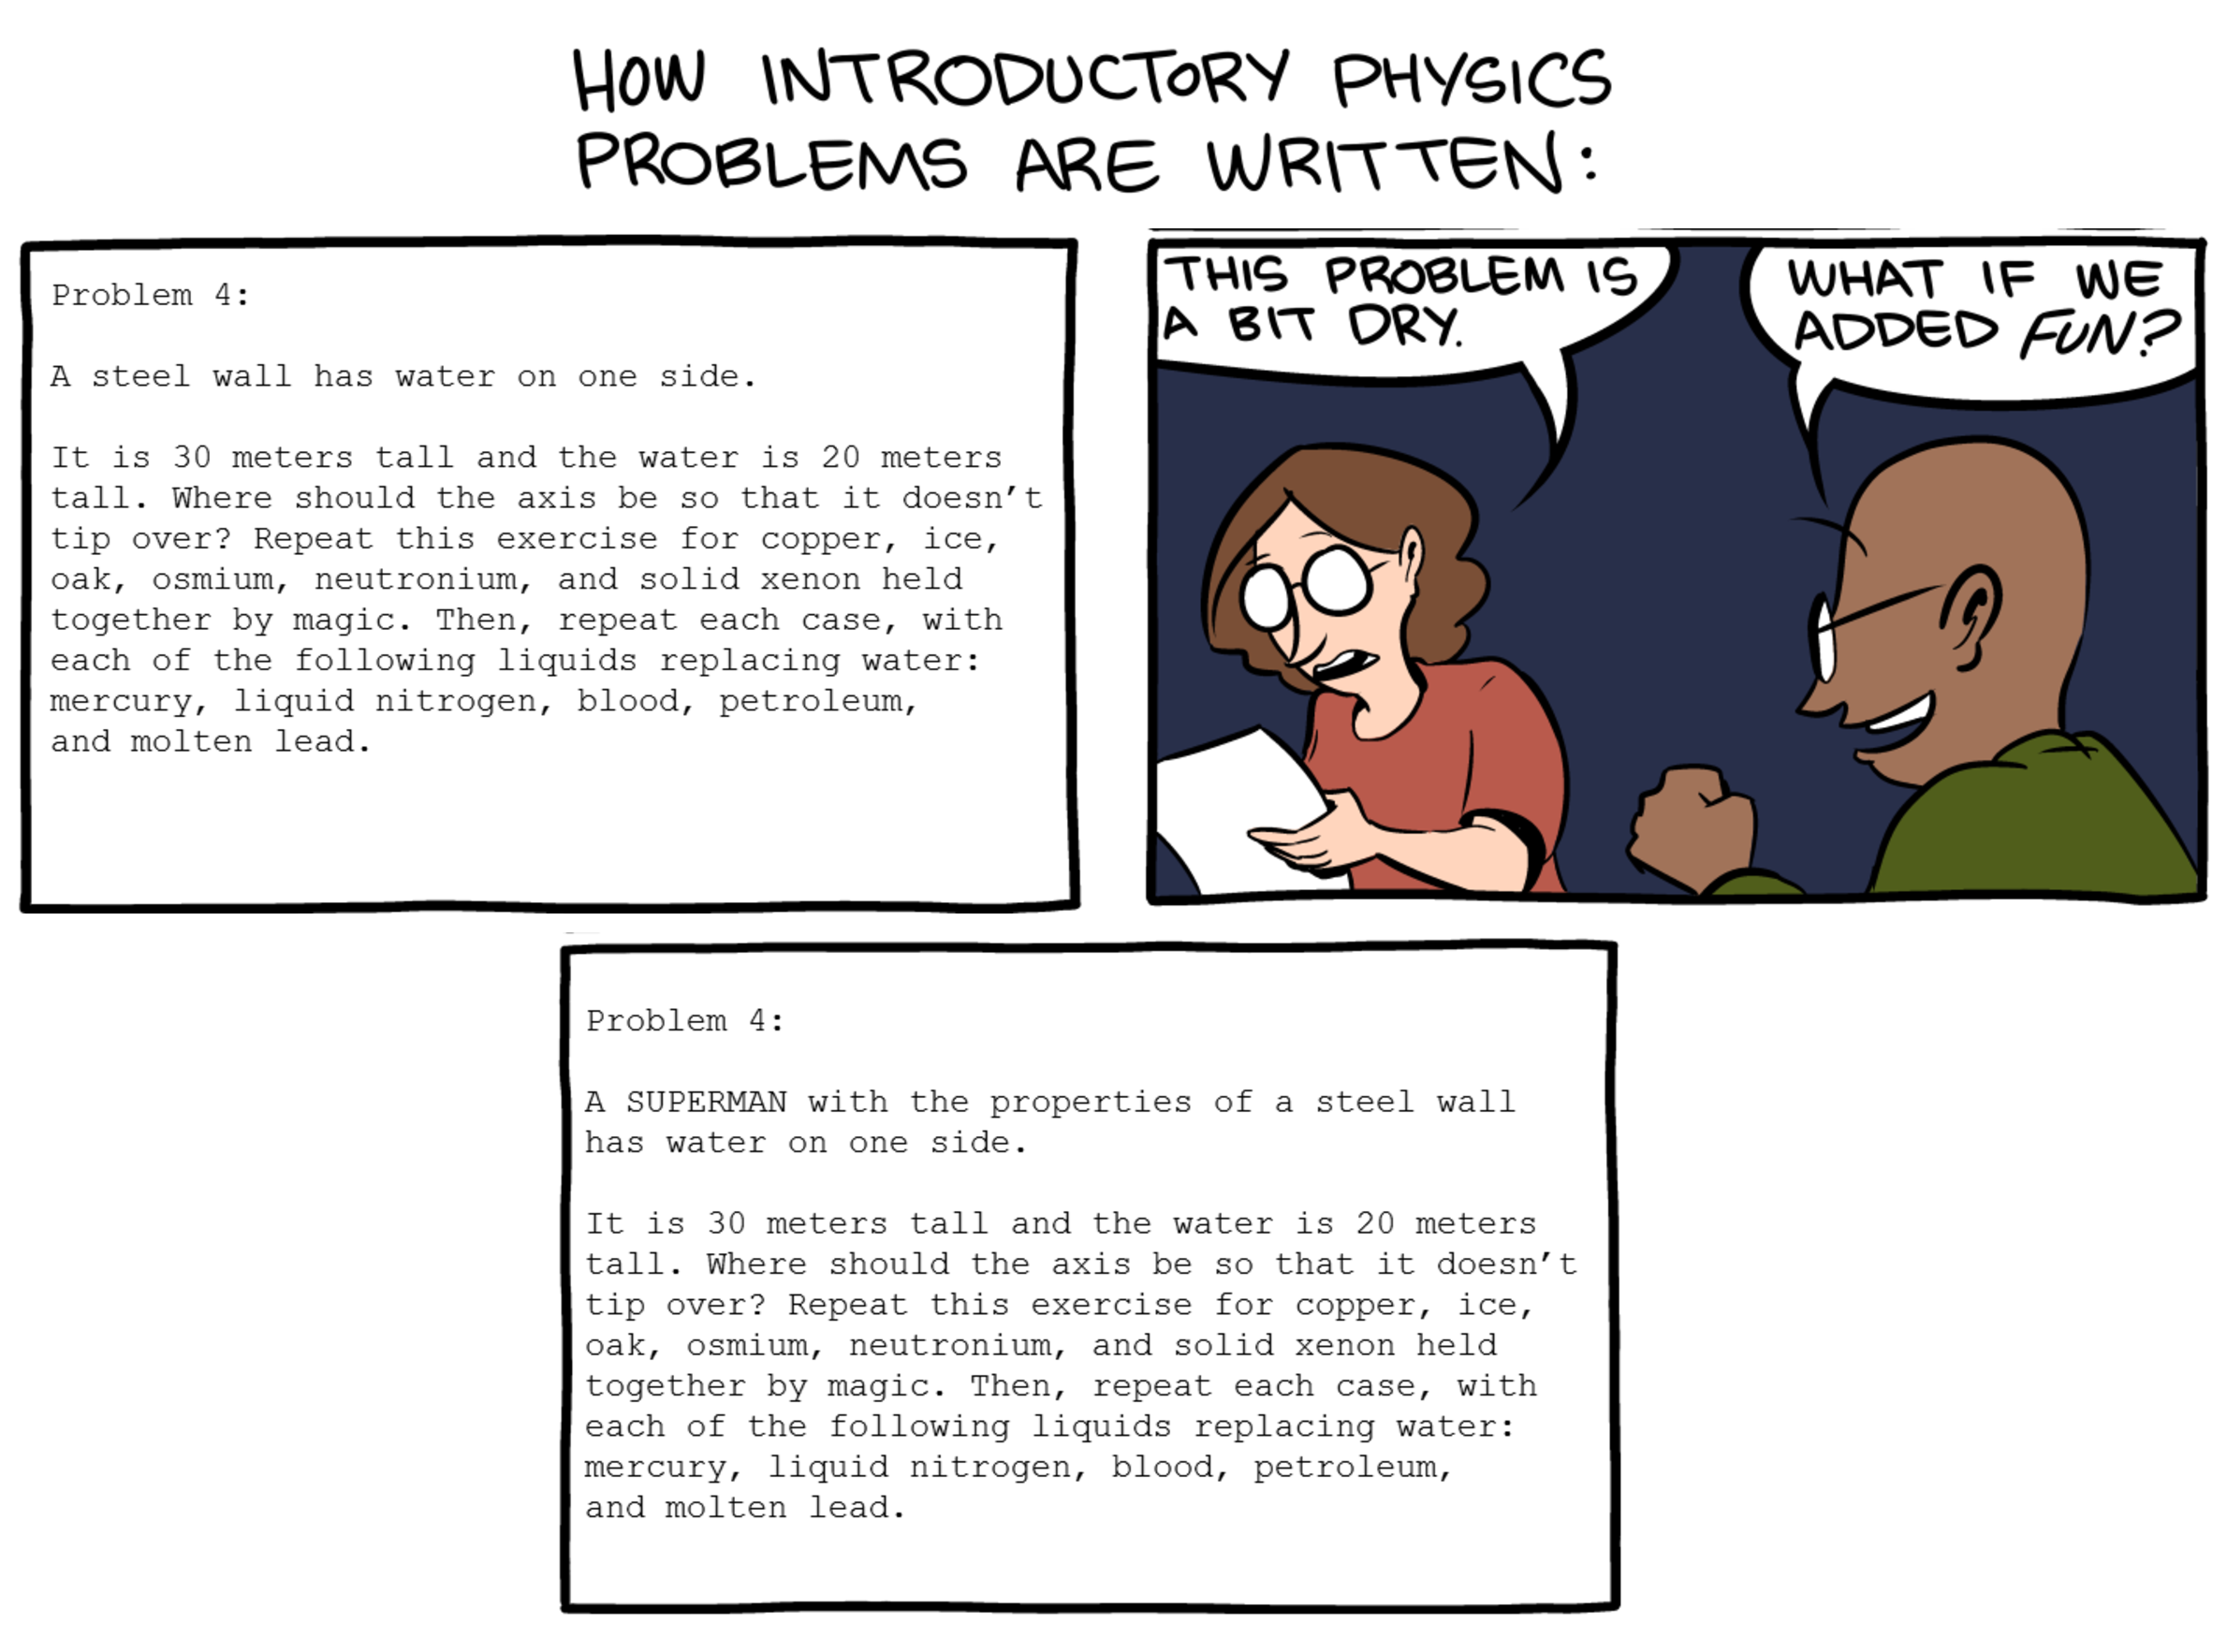
\psfig{file=images/smbc.eps, width=\linewidth}
	\end{center}
	\caption{Making the context ``Fun'' is not necessarily trivial, whether in physics education or computer science education.~\cite{SMBC}}
	\label{fig-comic-context}
\end{figure}

Of course, it is up to instructor to determine the depth and breadth of the context's integration.
The trade-off between the value and distraction added by the context is a delicate formula.
Consider the scenario in figure \ref{fig-comic-context}.
A steel wall is a relatively relatable concept for most students -- they can readily imagine such a large, durable object, and it somewhat reasonable to expect that objects would interfere with it.
In this scenario, the instructors consider replacing the wall with a comic book character -- something that they anticipate will be more ``fun''.
If they are in tune with their learners, this might actually be an effective context -- perhaps they know that their learners are comic book fans.
However, because the integration is only at the surface level, it is possible that the learners will see this as a forced reference, and they will have a more negative reaction.
It is also possible that they will not recognize the reference, or feel no positive emotions with it -- many contexts do not take into account gender, racial, or socio-economic characteristics of the anticipated learner.


\subsection{Theories of Motivation}

Theories of learning are distinctive from theories of motivation; the former determines how learning occurs, but the latter determines if and why learning occurs.
Situated Learning Theory, Constructivism, and other theories of learning have implications for how people choose to engage in the learning process, but they are not sufficient in themselves.
Instead, it is useful to turn to the dedicated motivational models as a lens to explore why people choose to participate and excel in Computer Science.
In this preliminary proposal, we lean on the MUSIC Model of Academic Motivation as a primary framework.

\subsubsection{MUSIC Model of Academic Motivation}

The decision to use the MUSIC model was based on several criteria.
Although there are many motivational models available, few strive to be holistic models specifically developed for academics.
For example, theories like Expectancy-Value and Cognitive Evaluation Theory have a wider scope and have stemmed from other disciplines such as healthcare.
The MUSIC Model is derived from a meta-analysis of these other theories, incorporating only the academically relevant components.
Further, the MUSIC model is a tool meant for both design and evaluation, allowing it to be used in all phases of this work.
Finally, the model and its associated instrument, the MUSIC Model of Academic Motivation Inventory (MMAMI) , has been extensively validated and utilized in other educational domains, making it a reliable device\cite{jones-validity}.

The MUSIC model identifies five key constructs in motivating students \cite{jones-description}:
\begin{description}
	\item[eMpowerment:] The amount of control that a student feels that they have over their learning -- e.g., course assignments, lecture topics, etc..
	\item[Usefulness:] The expectation of the student that the material they are learning will be valuable to their short and long term goals. There is no clear delineation of the time-scale for these goals, but there is nonetheless a distinction between strategic skills that students need to be successful in careers and personal interests and the tactical skills they need to complete present-day tasks.
	\item[Success:] The student's belief in their own ability to complete assignments, projects, and other elements of a course with the investment of a reasonable, fulfilling amount of work.
	\item[Interest:] The student's perception of how the assignment appeals to situational or long-term interests. The former covers the aspects of a course related to attention, while the latter covers topics related to the fully-identified areas of focuses of the student.
	\item[Caring:] The students perception of other stakeholders' attitudes toward them. These stakeholders primarily include their instructor and classmates, but also can be extended to consider other members of their learning experience (e.g., administration, external experts, etc.).
\end{description}

Students are motivated when one or more of these constructs is sufficiently activated.
They are not all required to achieve maximal levels, and in fact that is not always desired -- it is possible, for instance, for a student to feel too empowered, and become overwhelmed by possibilities.
For some of these constructs, a careful balance is required, and it may not be possible to ever achieve a minimal level; no matter how exciting you make your lecture, you may never convince your students it is interesting, although it is possible that they will still consider it useful and stay motivated.
Much like in Situated Learning Theory, students' subjective \textit{perception} of these constructs is a defining requirement and is more important than objective reality.

The MUSIC model is often used as an organizational framework and an evaluative tool.
As the former, it is a list of factors to consider when building modules, assignments, and content of a course.
At all times, instructors can consider whether they are leveraging at least one construct to motivate their students.
As the latter, it offers both a quantified instrument (MMAMI) and a structure to anchor a qualitative investigation on.
The model has also directly been used tactically in course design: Jones describes a controlled classroom experiment to motivate students by having an experimental group reflect on how a course satisfies the constructs of the MUSIC model (e.g., prompted to answer ``How will the material presented here will be useful to you?'').
Quantitative data gathered after the experiment indicated a significant increase in motivation.~\cite{mcginley2014brief}

\subsubsection{Other Models}

Although the MUSIC Model is a holistic model, it can be useful to explore other theories of motivation that it draws on.
Self-efficacy is just such a theory, concerned with a learners judgment of their own capabilities.
Self-efficacy is often a strong predictor of students performance.
Students that believe they will fail will often do so, despite whatever ability they may have.
Self-regulation is another such model, explaining how students approach the learning process.
Self-regulated learners will work earlier, more often, and more intelligently to solve problems.
They know when to get help, and how to ask for it.
Unfortunately, self-regulatory abilities are in short supply.
There are many other theories that are worth exploring.

\subsubsection{Extrinsic Motivation}

Although ideally, students will always be internally motivated to learn new subjects, this isn't always the case.
Academics are a careful balance of extrinsic and intrinsic motivation, with both internal and external rewards.
For instance, the ultimate goal of most formal education is certification, either by an accredited university or some other independent body.
In order to keep students on task, positive and negative grades are assigned based on performance.
Although these grades can drive negative behavior (e.g., nit-picking, arguments, etc.), they are ultimately necessary for some class of learners.
It can be a serious challenge for instructors to assign grades and use other forms of extrinsic motivation, to avoid dragging students along in a rigid environment but also not preventing students from floundering.
Too loose with a grading scheme, and students may deprioritize a course over stricter ones.
Too hard, and students may feel overwhelmed.
Although my research will not focus much on extrinsic motivation, it is important to understand its role in the classroom experience.